%% Classe du document
\documentclass{beamer}

%% Francisation
\usepackage[francais]{babel} % Indique que l'on utilise le francais
\usepackage[T1]{fontenc}
\usepackage[utf8]{inputenc} % Indique que l'on utilise tout le clavier

%% Define color
\definecolor{DeepSkyBlue3}{RGB}{0, 178, 238}
\definecolor{violet}{RGB}{202, 225, 255}
\definecolor{DeepSkyBlue4}{RGB}{0, 104, 139}
\definecolor{SteelBlue1}{RGB}{99, 184, 255}

%% Choix du thème
\usetheme{Darmstadt}
\mode<presentation>

\setbeamertemplate{navigation symbols}{}
\setbeamercovered{transparent}
%% Change color
\setbeamercolor{palette primary}{use={structure,normal text},fg=white,bg=DeepSkyBlue3} %theme
\setbeamercolor{palette secondary}{use={structure,normal text},fg=white,bg=SteelBlue1}%theme
\setbeamercolor{palette tertiary}{use={structure,normal text},fg=white,bg=violet} % theme
\setbeamercolor{palette quaternary}{use={structure,normal text},fg=structure.fg,bg=violet} % theme
\setbeamercolor{example text}{fg=DeepSkyBlue4}

\title{Making the Local-As-View approach feasible in Semantic Web and Application with Open Data and DBpedia}
%\subtitle{bloup}
\author{COUTABLE Guillaume, GAUTIER Gaëtan, RULLIER Noémie}

\begin{document}

\begin{frame}
\titlepage
\end{frame}

%%%%%%%%%%%%%%%%%%%%%%%%%%%%%%%%%%%%%%%%%%%%%%%%%%%%%%%%%%%%%%%%%%%%%%%%%%%%%
%%%%%%%%%%  Table de matieres
%%%%%%%%%%%%%%%%%%%%%%%%%%%%%%%%%%%%%%%%%%%%%%%%%%%%%%%%%%%%%%%%%%%%%%%%%%%%%
\begin{frame}
\frametitle{Table of contents}
\tableofcontents
\end{frame}

%%%%%%%%%%%%%%%%%%%%%%%%%%%%%%%%%%%%%%%%%%%%%%%%%%%%%%%%%%%%%%%%%%%%%%%%%%%%%
%%%%%%%%%%  Introduction générale
%%%%%%%%%%%%%%%%%%%%%%%%%%%%%%%%%%%%%%%%%%%%%%%%%%%%%%%%%%%%%%%%%%%%%%%%%%%%%
\section{Introduction}
\begin{frame}
\frametitle{Introduction}
\begin{center}
\begin{itemize}
\item Web semantic and open data
\begin{itemize}
\item Lots of data
\item Need to query
\end{itemize}
\item Data integration
\begin{itemize}
\item Warehousing
\item Mediation (GAV and LAV)
\begin{itemize}
\item Rewriting algorithm (Bucket, Minicon)
\end{itemize}
\end{itemize}
\end{itemize}
\end{center}
\end{frame}

\begin{frame}
\frametitle{Data integration}
\framesubtitle{Warehousing}
\begin{center}
\begin{itemize}
\item The data sources are aggregated into a global basis
\item The sources are not interviewed in a query
\end{itemize}
\uncover<2>{\begin{block}{Difficulties}
\begin{itemize}
\item Effectively detect and perform the update of data
\item Not applicable to a large number of sources
\item Add new source
\end{itemize}
\end{block}}
\end{center}
\end{frame}

\begin{frame}
\frametitle{Data integration}
\framesubtitle{Mediation}
\begin{center}
The mediator asks necessary data sources to the query and assembles the sub-results.
\end{center}
\end{frame}

\begin{frame}
\frametitle{Data integration}
\framesubtitle{Mediation Global-As-View}
\begin{center}
The global schema was expressed according with the data sources.
\begin{example}
\begin{equation}
Product = Source 1 \cup Source 2
\end{equation}
\end{example}
\end{center}
\end{frame}

\begin{frame}
\frametitle{Data integration}
\framesubtitle{Mediation Local-As-View}
\begin{center}
\begin{itemize}
\item The data sources are expressed according with the global schema.
\item For each request, the mediator search the sources which can provide results. This allows the source to change regularly.
\end{itemize}
\begin{example}
\begin{equation}
Source 1 <\text{include or equal}> Products <\text{join}> Vendors
\end{equation}
\end{example}
\end{center}
\end{frame}

%%%%%%%%%%%%%%%%%%%%%%%%%%%%%%%%%%%%%%%%%%%%%%%%%%%%%%%%%%%%%%%%%%%%%%%%%%%%%
%%%%%%%%%%  Problématique
%%%%%%%%%%%%%%%%%%%%%%%%%%%%%%%%%%%%%%%%%%%%%%%%%%%%%%%%%%%%%%%%%%%%%%%%%%%%%
\section{Problematic}
\begin{frame}
\frametitle{Problematic}
\begin{center}
Making the Local-As-View approach feasible in Semantic Web
\end{center}
\end{frame}

%%%%%%%%%%%%%%%%%%%%%%%%%%%%%%%%%%%%%%%%%%%%%%%%%%%%%%%%%%%%%%%%%%%%%%%%%%%%%
%%%%%%%%%%  Solutions proposées
%%%%%%%%%%%%%%%%%%%%%%%%%%%%%%%%%%%%%%%%%%%%%%%%%%%%%%%%%%%%%%%%%%%%%%%%%%%%%
\section{Proposed solutions}
\begin{frame}
\frametitle{Proposed solutions}
\begin{center}
\begin{minipage}{0.69\textwidth}
        \begin{itemize}
\item GUN
	\begin{itemize}
	\item Detection of relevant views
	\item Rewritings only on those views
	\end{itemize}
\item SemLAV
	\begin{itemize}
	\item Abandonment of rewritings
	\item Immediate execution of view's body
	\end{itemize}
\item Comparison with other approaches
\end{itemize}
\end{minipage}
\begin{minipage}{0.29\textwidth}
	\begin{figure}
		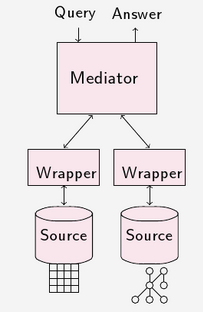
\includegraphics[width=3cm]{Images/Solutions.png}
	\end{figure}
\end{minipage}
\end{center}
\end{frame}

\begin{frame}
\frametitle{GUN}
\begin{center}
Main feature: only few rewritings are executed.
\begin{enumerate}
\item Use Bucket algorithm to calculate the relevant views
\item ???????????????
\end{enumerate}
\end{center}
\end{frame}

\begin{frame}
\frametitle{SemLAV}
\begin{center}
Improvment of GUN algorithm: no rewritings are executed.
\begin{enumerate}
\item Use Bucket algorithm to calculate the relevant views and build the buckets (No change here)
\item Storage of views based on the number of their appearances
\end{enumerate}
\alert{Consequence: The bulk of the result is calculate faster}
\end{center}
\end{frame}

\end{document}